\documentclass[../../main.tex]{subfiles}
\begin{document}
\section{Additional Tools}
A few tools remain to be explained before we can jump into the algorithm. These tools have a variety of reasons for being used that will be explained individually. 
\subsection{$k$-mer}
In order to create the sets that {\bf Mm½} and {\bf Mm} sketches are built with, we shall be using $k$-mer to partition each sequence into subsets. The $k$-mer of a sequence string are defined as follows:
\begin{center}
{\bf The $k$-mer of a sequence string $s$ is the set of all the substrings of size $k$ of $s$.}
\end{center}
The 1-mer of a sequence string, will therefore be the set of all characters in the sequence string. It is therefore sensible to consider the size of $k$ when partitioning the sequence string.
\subsubsection{$k$-mer transformation}
Given that the $k$-mers will be used as hash function input, it is reasonable to transform them to an input that is easy to map. As sequence strings only comprimise of 4 characters (A,C,G,T), we assign each character a 2 bit value so that $A=\mathbf{00},C=\mathbf{01},G=\mathbf{10},T/U=\mathbf{11}$, and then put them in sequence according to their position in the substring, eg.
\begin{figure}[h]
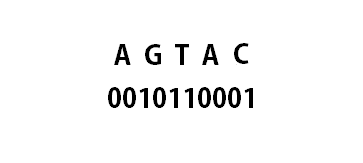
\includegraphics[scale=0.4]{fig/kmertransformed}
\end{figure}\\
which also greatly reduces the memory usage.
\subsection{MapReduce}
Given a sizeable amount of sequences per file, it was quite essential to have a parallel and distributed programming model. For this purpose, MapReduce is a popular programming model. It works by distributing its task to a multitude of workers. Worker can be computers or cores. It expresses its computation as two functions:
\begin{enumerate}
\item Map: Runs a function over each element of a list and returns an intermediate value.
\item Reduce: Merges the intermediate values to form a potentially smaller set of values.
\end{enumerate}

 As explained in \cite{mapreduceExplained}, MapReduce processes input by the following steps
\begin{enumerate}
\item Map step: Splits the input into $M$ splits. Each split is then distributed to a worker who will perform a Map function on the given split and saves the result into a temporary storage.
\item Shuffle step: The results from the Map calls are then written to a local disk, partitioned into $R$ regions.
\item Reduce step: For each region, a worker is set to run a Reduce job on it, in parallel.
\end{enumerate}

MapReduce has been shown to scaler better than other parallel programming tools for input sizes that surpass 100 Mb, which is why it chosen.\cite{compForkMapRed} Apache Hadoop MapReduce was used, as it is free source. However, since the startup time of Hadoop MapReduce is around 4 seconds, MapReduce is directly slower at small input files.

\subsection{Pig}
Pig Latin is a high level language for compiling and executing MapReduce jobs over Hadoop. Advantageous when performing a pipeline of MapReduce jobs\cite{pig}, it also demands very few lines of code compared to Hadoop MapReduce code. Additionally, users may write User Defined Functions (abbr. UDF), completely eliminating the need to write any map or reduce function, as they are on the lower level.


 
\end{document}

